\section{Volumes of Revolution}
As we did for areas between curves, we can use our knowledge of
integrals to compute the volume of certain objects: ones obtained
by rotating a region about a horizontal or vertical line!

\begin{Remark}{}{}
    For more general shapes, we need multivariable methods. These are
    explored in MATH 237!
\end{Remark}

Let's get a formula!

\underline{Areas}:
\begin{itemize}
    \item Area of one infinitesimally thin rectangle: $ f(x)\,dx $
    \item Overall area: $ \displaystyle \int_{a}^{b} f(x)\, d{x}  $
\end{itemize}
\underline{Volumes} (rotate $ f $ around $ x $-axis):
\begin{itemize}
    \item Volume of one infinitesimally thin slice: $ A(x)\,dx $
    \item Overall volume: $ \displaystyle \int_{a}^{b} A(x)\, d{x} $
\end{itemize}

So, we just need to determine $ A(x) $ in each case! There are
a few different methods we will use.

The two main methods are:
\begin{enumerate}[label=(\Roman*)]
    \item Washers/disks (i.e.\ cross-sections)
    \item Cylindrical shells
\end{enumerate}

\subsection*{Method 1: Washers/disks}

First, let's recall the area formulas:

\begin{figure}
    \centering
    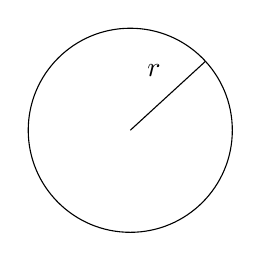
\begin{tikzpicture}[x=0.75pt,y=0.75pt,yscale=-1,xscale=1]
        %uncomment if require: \path (0,123); %set diagram left start at 0, and has height of 123

        %Shape: Circle [id:dp2971916951811683] 
        \draw   (31,59.83) .. controls (31,32.68) and (53.01,10.67) .. (80.17,10.67) .. controls (107.32,10.67) and (129.33,32.68) .. (129.33,59.83) .. controls (129.33,86.99) and (107.32,109) .. (80.17,109) .. controls (53.01,109) and (31,86.99) .. (31,59.83) -- cycle ;
        %Straight Lines [id:da8239626600891564] 
        \draw    (80.17,59.83) -- (116.33,26.67) ;

        % Text Node
        \draw (87.17,26.9) node [anchor=north west][inner sep=0.75pt]    {$r$};
    \end{tikzpicture}
    \caption{Area of a disk with radius $ r $: $ \pi r^2 $}
\end{figure}

\begin{figure}
    \centering
    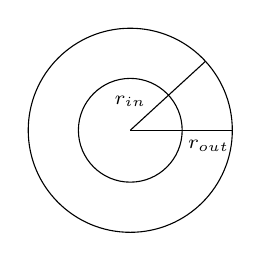
\begin{tikzpicture}[x=0.75pt,y=0.75pt,yscale=-1,xscale=1]
        %uncomment if require: \path (0,123); %set diagram left start at 0, and has height of 123

        %Shape: Circle [id:dp2971916951811683] 
        \draw   (31,59.83) .. controls (31,32.68) and (53.01,10.67) .. (80.17,10.67) .. controls (107.32,10.67) and (129.33,32.68) .. (129.33,59.83) .. controls (129.33,86.99) and (107.32,109) .. (80.17,109) .. controls (53.01,109) and (31,86.99) .. (31,59.83) -- cycle ;
        %Straight Lines [id:da8239626600891564] 
        \draw    (80.17,59.83) -- (116.33,26.67) ;
        %Shape: Circle [id:dp7459673192558707] 
        \draw   (55.17,59.83) .. controls (55.17,46.03) and (66.36,34.83) .. (80.17,34.83) .. controls (93.97,34.83) and (105.17,46.03) .. (105.17,59.83) .. controls (105.17,73.64) and (93.97,84.83) .. (80.17,84.83) .. controls (66.36,84.83) and (55.17,73.64) .. (55.17,59.83) -- cycle ;
        %Straight Lines [id:da52555392875757] 
        \draw    (129.33,59.83) -- (80.17,59.83) ;

        % Text Node
        \draw (106.75,63.23) node [anchor=north west][inner sep=0.75pt]  [font=\scriptsize]  {$r_{\text{out}}$};
        % Text Node
        \draw (80.17,42) node [anchor=north] [inner sep=0.75pt]  [font=\scriptsize]  {$r_{\text{in}}$};


    \end{tikzpicture}
    \caption{Area of a washer with outer radius $ r_{\text{out}} $ and inner radius $ r_\text{in} $:
        $ \pi(r_{\text{out}})^2-\pi(r_\text{in})^2 $}
\end{figure}


\begin{Example}{}{}
    Find the volume of the solid obtained by rotating $ f(x)=\sqrt{x-1} $ about the $ x $-axis
    from $ x=1 $ to $ x=5 $.

    \begin{center}
        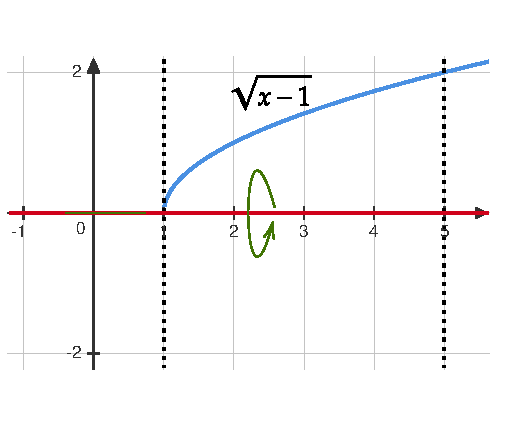
\includegraphics[width=0.45\textwidth]{diagram 21.pdf}
        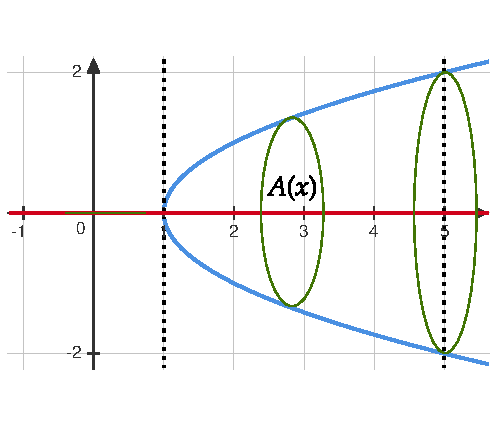
\includegraphics[width=0.45\textwidth]{diagram 22.pdf}
    \end{center}

    \textbf{Solution.} The cross-section is a disk with radius $ \sqrt{x-1} $. So
    \[ A(x)=\pi\left( \sqrt{x-1} \right)^2=\pi(x-1) \]
    and
    \begin{align*}
        \text{Volume}
         & =\int_{1}^{5} A(x)\, d{x}                         \\
         & =\int_{1}^{5} \pi(x-1)\, d{x}                     \\
         & =\pi\left[ \frac{x^2}{2} -x \right]_1^5           \\
         & =\pi\left( \frac{25}{2} -5-\frac{1}{2} +1 \right) \\
         & =8\pi
    \end{align*}
\end{Example}

Note that you don't need to draw the full 3-D image, just one area slice is enough!

\begin{Example}{}{}
    Rotate the area between $ y=\sqrt{x} $ and $ y=x^2 $ about the line $ y=1 $.

    \begin{center}
        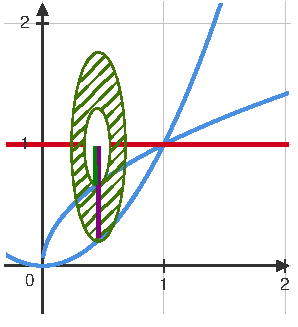
\includegraphics[width=0.6\textwidth]{diagram 3.pdf}
    \end{center}

    \textbf{Solution.} The cross-section is a washer with $ \color[rgb]{0.5,0,0.5}r_{\text{out}}=1-x^2 $ and
    $ \color[rgb]{0,0.5,0} r_{\text{in}}=1-\sqrt{x} $. So,
    \begin{align*}
        A(x)
         & =\pi(r_{\text{out}})^2-\pi(r_\text{in})^2   \\
         & =\pi\left[ (1-x^2)^2-(1-\sqrt{x})^2 \right] \\
         & =\pi(1-2x^2+x^4-1+2\sqrt{x}-x)              \\
         & =\pi(x^4-2x^2+2\sqrt{x}-x)
    \end{align*}
    and
    \begin{align*}
        \text{Volume}
         & =\int_{0}^{1} A(x)\, d{x}                                                                        \\
         & =\pi \int_{0}^{1} x^4-2x^2+2x^{\sfrac{1}{2}}-x\, d{x}                                            \\
         & =\pi\left[ \frac{x^5}{5} -\frac{2}{3} x^3+\frac{4}{3} x^{\sfrac{3}{2}}-\frac{x^2}{2} \right]_0^1 \\
         & =\pi\left( \frac{1}{5} -\frac{2}{3} +\frac{4}{3} -\frac{1}{2} \right)                            \\
         & =\frac{11\pi}{30}
    \end{align*}
\end{Example}


\begin{Example}{}{}
    Rotate the region between $ x=y^2 $ and $ x=2y $ about the $ y $-axis.

    \begin{center}
        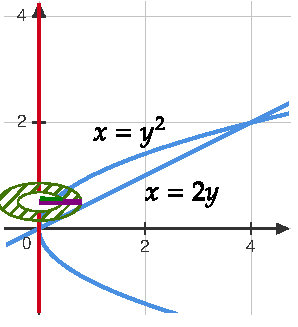
\includegraphics[width=0.6\textwidth]{diagram 4.pdf}
    \end{center}

    \textbf{Solution.} First, points of intersection: $ y^2=2y\implies y=0,2 $.
    The cross-section is a washer with $ \color[rgb]{0.5,0,0.5} r_{\text{out}}=2y $ and
    $ \color[rgb]{0,0.5,0}  r_{\text{in}}=y^2 $. So,
    \begin{align*}
        A(y)
         & =\pi\left(2y\right)^2-\pi\left(y^2\right)^2 \\
         & =\pi\left( 4y^2-y^4 \right)
    \end{align*}
    and
    \begin{align*}
        \text{Volume}
         & =\pi \int_{0}^{2} 4y^2-y^4\, d{y} \\
         & =\text{exercise}                  \\
         & =\frac{64\pi}{15}
    \end{align*}
\end{Example}

We can see that washers/disks arise when we rotate functions of $ x $ about
a horizontal line or functions of $ y $ about a vertical line.

We can't use it all the time though, for example: rotate the region below
$ y=2x^2-x^3 $ about the $ y $-axis from $ x=0 $ to $ x=2 $.

\begin{center}
    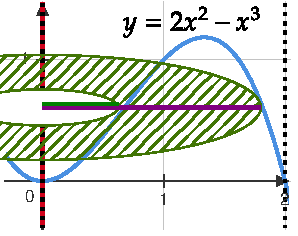
\includegraphics[width=0.6\textwidth]{diagram 5.pdf}
\end{center}

We need another method!

\subsection*{Method 2: Cylindrical shells}

Instead of using cross-sections, we can use cylindrical shells (think soup can labels)
to divide the volume up!

Q\@: What is the area of a cylindrical shell with base radius $ r $ and height $ h $?

\begin{center}
    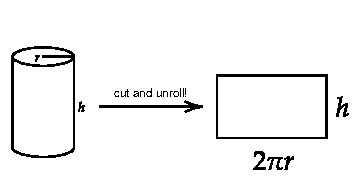
\includegraphics[width=0.6\textwidth]{diagram 6.pdf}
\end{center}

So area is $ 2\pi rh $. So, we only need to determine $ r $ and $ h $!

Back to the difficult example:
\begin{Example}{}{}
    Rotate the region below $ y=2x^2-x^3 $ about the $ y $-axis from $ x=0 $ to $ x=2 $.
    \begin{center}
        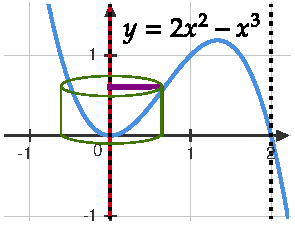
\includegraphics[width=0.6\textwidth]{diagram 7.pdf}
    \end{center}
    \textbf{Solution.} The area is a cylindrical shell with radius $ r=x $ and height
    $ h=2x^2-x^3 $. So,
    \[ A(x)=2\pi x\left( 2x^2-x^3 \right) \]
    and
    \[ \text{Volume}=\int_{0}^{2}2\pi x\left( 2x^2-x^3 \right)\, d{x} \]
\end{Example}

\begin{Example}{}{}
    Find the volume in each case.
    \begin{enumerate}[label=(\roman*)]
        \item Rotate the region between $ y=x^2 $ and $ y=6x-x^2 $
              about the $ y $-axis.



              \textbf{Solution.} Intersection points:
              $ x^2=6x-2x^2\implies x=0,2 $
              \begin{itemize}
                  \item $ r=x $
                  \item $ h=6x-2x^2-x^2=6x-3x^2 $
              \end{itemize}
              \[ A(x)=2\pi x\left( 6x-3x^2 \right) \]
              \begin{align*}
                  V
                   & =\int_{0}^{2} 2\pi x\left( 6x-3x^2 \right)\, d{x} \\
                   & =2\pi \int_{0}^{2} 6x^2-3x^3\, d{x}               \\
                   & =2\pi\left[ 2x^3-\frac{3}{4} x^4 \right]_0^2      \\
                   & =2\pi\left( 16-12 \right)                         \\
                   & =8\pi
              \end{align*}
        \item Rotate the region bounded by $ y=4x-x^3 $ and $ y=3 $ about
              $ x= 1 $.

              \textbf{Solution.} Intersection points:
              $ 4x-x^2=3\implies x=1,3 $
              \begin{itemize}
                  \item $ r=x-1 $
                  \item $ h=4x-x^3-3 $
              \end{itemize}
              \[ A(x)=2\pi(x-1)(4x-x^2-3) \]
              \begin{align*}
                  V
                   & =\int_{1}^{3}2\pi(x-1)(4x-x^2-3) \, d{x} \\
                   & =\text{exercise}                         \\
                   & =\frac{8\pi}{3}
              \end{align*}
    \end{enumerate}
\end{Example}

We will now look at some more practice examples, but first a handy table:

\begin{table}[H]
    \centering
    \begin{tabularx}{0.7\linewidth}{@{}YYY@{}}
                        & Functions of $ x $ & Functions of $ y $ \\
        \midrule
        Vertical line   & Cylindrical shells & Washers/disks      \\
        Horizontal line & Washers/disks      & Cylindrical shells
    \end{tabularx}
\end{table}

\begin{Example}{More Practice}{}
    Set up, but don't evaluate the integral(s) that would give
    the desired volume.

    \begin{enumerate}[label=(\roman*)]
        \item Rotate the region bounded by $ xy=1 $, $ x=0 $, $ y=1 $, $ y=3 $,
              around the $ x $-axis.

              \textbf{Solution 1.} Cylindrical shell:
              \begin{itemize}
                  \item $ r=y $
                  \item $ h=\sfrac{1}{y} $
              \end{itemize}
              \[ A(y)=2\pi y\left( \frac{1}{y}  \right)=2\pi \]
              \[ V=\int_{1}^{3} 2\pi\, d{y}=4\pi \]
              \textbf{Solution 2.} For fun, can we do it using washers/disks?

              A\@: Yes! Just work with $ x $ and not $ y $.
              \begin{itemize}
                  \item $ \displaystyle  r_{\text{out}}=\begin{cases}
                                3            & 0\leqslant x\leqslant \sfrac{1}{3}   \\
                                \sfrac{1}{x} & \sfrac{1}{3} \leqslant x \leqslant 1
                            \end{cases} $
                  \item $ r_{\text{in}}=1 $
              \end{itemize}
              \begin{align*}
                  V
                   & =\int_{0}^{\sfrac{1}{3}} \pi(3)^2-\pi(1)^2\, d{x}
                  +\int_{\sfrac{1}{3}}^{1} \pi\left( \frac{1}{x} \right)^2-\pi(1)^2\, d{x}
              \end{align*}
              This method was more difficult, because $ r_{\text{out}} $ changes but it is still valid!

        \item Region bounded by $ x=(y-1)^2 $, $ x=y+1 $, about $ x=-1 $.

              \textbf{Solution.} Points of intersection:
              \[ (y-1)^2=y+1\implies y=0,3 \]
              \begin{itemize}
                  \item $ r_{\text{out}}=y+1-(-1)=y+2 $
                  \item $ r_{\text{in}}=(y-1)^2-(-1)=(y-1)^2+1 $
              \end{itemize}
              \[ V=\pi \int_{0}^{3} (y+2)^2-\left[ (y-1)^2+1 \right]^2\, d{y}  \]
    \end{enumerate}
\end{Example}

\chapter{Differential Equations}
\section{Introduction to Differential Equations}
\begin{Definition}{Ordinary Differential Equation}{}
    An equation containing derivatives of a dependent variable (i.e.\ function) $ y=f(x) $
    is called an \textbf{ordinary differential equation} (ODE).
\end{Definition}

\begin{Remark}{}{}
    To contrast, there are also partial differential equations for multivariable functions.
\end{Remark}

\begin{Example}{Ordinary Differential Equations}{}
    \begin{itemize}
        \item $ y^\prime+2y=e^x $
        \item $ y^{\prime\prime}+y^\prime+y=0 $
        \item $ x^2y^\prime+y=31 $
    \end{itemize}
\end{Example}

\begin{Definition}{Order}{}
    The \textbf{order} of an ODE is the order of the highest derivative that appears.
\end{Definition}

\begin{Example}{Order}{}
    \begin{itemize}
        \item $ y^{\prime\prime}+y^3=0 $: order 2
        \item $ x^2 \frac{d^2y}{dx^2} +\frac{dy}{dx} =y $: order 2
        \item $ y^\prime+y=\sin(x) $: order 1
    \end{itemize}
\end{Example}

\begin{Definition}{Linear}{}
    An ODE is called \textbf{linear} if it contains only linear functions in $ y $, $ y^\prime $,
    $ y^{\prime\prime} $, etc.
\end{Definition}

\begin{Example}{Linear and Non-linear ODEs}{}
    \begin{itemize}
        \item $ 3y^{\prime\prime}+2x^3y=\cos(x) $: linear
        \item $ y^2+y^\prime=0 $: not linear $ (y^2) $
        \item $ yy^\prime=0 $: not linear
    \end{itemize}
\end{Example}

\begin{Definition}{General Solution}{}
    The \textbf{general solution} of an ODE is the collection fo all possible
    solutions including arbitrary constants.
\end{Definition}

\begin{Definition}{Particular Solution}{}
    A \textbf{particular solution} is a solution in which all arbitrary constants
    have been determined.
\end{Definition}

\begin{Definition}{Initial Conditions}{}
    To get a particular solution, we would need some additional info, like values of $ y $,
    $ y^\prime $, $ y^{\prime\prime} $, etc.\ for certain $ x $-values. These are
    called \textbf{initial conditions}.
\end{Definition}

An ODE together with initial conditions is called an \textbf{initial value problem} (IVP).

In general, solving ODEs is difficult.
\begin{Example}{}{}
    \begin{itemize}
        \item $ y^{\prime}=x-y^2 $: impossible to solve
        \item $ y^\prime=y-x^2 $: easy to solve (next week!)
    \end{itemize}
\end{Example}

Soon, we will learn some techniques to solve certain ODEs, but for now we can
only find some simple solutions.

\begin{Example}{}{}
    What constant functions satisfy
    \[ y^\prime=y^3+2y^2-80y \]
    \textbf{Solution.} If $ y=C $, a constant, then $ y^\prime=0 $, so we can get
    \[ 0=C^3+2C^2-80C=C(C+10)(C-8) \]
    Therefore, $ C=0,-10,8 $. $ C $ is also known as \textbf{equilibrium solutions}.
\end{Example}
